
\begin{figure}
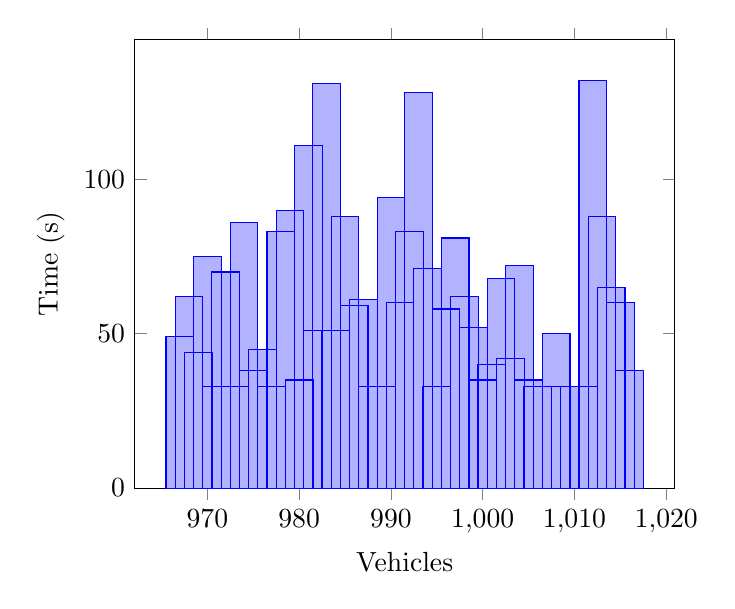
\begin{tikzpicture}
\begin{axis}[
legend style={anchor=west},
xlabel=Vehicles,
ylabel=Time (s),
ymin=0,
ybar,
]
\addplot coordinates {
(1005, 35)
(1014, 65)
(1015, 60)
(1016, 38)
(1010, 33)
(1011, 33)
(994, 71)
(1013, 88)
(1002, 68)
(1006, 33)
(972, 70)
(1009, 33)
(1008, 50)
(1007, 33)
(1004, 72)
(1000, 35)
(977, 33)
(976, 45)
(975, 38)
(974, 86)
(973, 33)
(971, 33)
(970, 75)
(979, 90)
(978, 83)
(1012, 132)
(995, 33)
(997, 81)
(996, 58)
(991, 60)
(990, 94)
(993, 128)
(992, 83)
(999, 52)
(998, 62)
(1003, 42)
(967, 49)
(968, 62)
(969, 44)
(988, 33)
(989, 33)
(982, 51)
(983, 131)
(980, 35)
(981, 111)
(986, 59)
(987, 61)
(984, 51)
(985, 88)
(1001, 40)
};

\end{axis}
\end{tikzpicture}
\label{tik:time:100:90}
\caption{100 percent diving with GSC on route $90$}
\end{figure}
